\ExerciseChapter{生存分析与Cox回归}

\label{chapter:3}

\par\addvspace{8pt}\noindent\begin{minipage}{\linewidth}

\section{作业题}

\subsection{数据分析题}

\Question{H3-1}{肺癌治疗的生存分析}

比较两种治疗疗法对延长肺癌患者存活时间的效果。观察了40例接受标准治疗和试验疗法的病人，同时记录患者年龄、病程、病理类型等信息。具体数据见 survivalhomework1。\textbf{共7分。}

变量：time（生存时间，天），status（死亡1、删失0），treat（标准疗法0、试验疗法1），age（年龄），coursetime（病程），type（病理类型：1鳞状、2小型、3腺状、4大型）。

\begin{enumerate}
\def\labelenumi{\arabic{enumi}.}
\tightlist
\item
  绘制并比较两个治疗组的生存曲线。（1分）
\item
  在控制年龄、病程和病理类型之后，比较两个治疗组的疗效。（1.5分）
\item
  哪些因素影响患者的存活时间？（1分）
\item
  如何评价所使用的模型是否合适？所构建的模型是较优的？（2分）
\item
  如何解释结果？不同治疗方法的疗效比较结果为差异没有统计学意义时，如何理解？（1.5分）
\end{enumerate}


\worklines{3}

\end{minipage}\par\vspace{5pt}

\par\addvspace{8pt}\noindent\begin{minipage}{\linewidth}

\subsection{文献分析题}

\Question{H3-2}{hsCRP与死亡风险：文献分析}

阅读 \emph{Mortality risk prediction of high-sensitivity C-reactive protein in suspected acute coronary syndrome: A cohort study}（附原文 pmed.1003911）。\textbf{共3分。}

\begin{enumerate}
\def\labelenumi{\arabic{enumi}.}
\tightlist
\item
  请凝练本篇文章要解决的科学问题。（0.5分）
\item
  原始数据结构主要包括了哪些变量？变量类型如何？（1分）
\item
  这篇文章的流行病学设计是什么？基于此设计，请简述如何用统计模型（Cox回归模型）来解决科学问题。（1.5分）
\end{enumerate}


\worklines{3}

\end{minipage}\par\vspace{5pt}

\par\addvspace{8pt}\noindent\begin{minipage}{\linewidth}

\section{往年题}

\subsection{单项选择题}

\Question{R24-M13}{乘积极限法的计算}

某随访资料在两个事件时刻的风险人数分别为5人、3人，事件数分别为2人、1人。在第二个事件时刻之后，Kaplan--Meier生存率估计为多少？


\begin{choices}

\item 0.20。

\item 0.30。

\item 0.40。

\item 0.60。

\item 0.80。

\end{choices}

\end{minipage}\par\vspace{5pt}

\par\addvspace{8pt}\noindent\begin{minipage}{\linewidth}

\Question{R24-M4}{事件与删失的排序}

采用Kaplan--Meier法估计生存率时，下列说法错误的是：


\begin{choices}

\item 将生存时间由小到大排序，完全数据与删失数据同一时刻发生时，删失数据排在完全数据前面。

\item 按不同事件时刻确定风险集。

\item 同一记录时刻既有事件又有右删失时，常规约定先计事件，再移除删失者。

\item 未发生事件的右删失者，其删失前的观察信息可以利用。

\item 估计生存率时，不需要先指定生存时间服从某个参数分布。

\end{choices}

\end{minipage}\par\vspace{5pt}

\par\addvspace{8pt}\noindent\begin{minipage}{\linewidth}

\Question{R24-M5}{生存曲线检验的权重}

按课程中对Log-rank检验与Breslow广义Wilcoxon检验的相对比较，下列哪项正确？


\begin{choices}

\item Log-rank检验对近期效应更敏感。

\item Log-rank检验对远期效应更敏感。

\item Breslow检验对远期效应更敏感。

\item 两者对近期效应同样敏感。

\item 两者对远期效应同样敏感。

\end{choices}

\end{minipage}\par\vspace{5pt}

\par\addvspace{8pt}\noindent\begin{minipage}{\linewidth}

\Question{R24-M6}{比例风险与时间}

同一未分层Cox比例风险模型中，两个个体的协变量均不随时间变化，且模型满足PH假设。在风险函数有定义的时刻，两者风险函数之比与时间的关系是：


\begin{choices}

\item 随时间线性增大。

\item 随时间指数减小。

\item 必定始终等于1。

\item 是与时间无关的常数，但不一定等于1。

\item 只要基线风险随时间变化，风险比就一定随时间变化。

\end{choices}

\end{minipage}\par\vspace{5pt}

\par\addvspace{8pt}\noindent\begin{minipage}{\linewidth}

\Question{R24-M10}{删失与终点事件}

以肝癌死亡为研究终点，进行肝癌患者随访研究时，下列情况不属于删失数据的是：


\begin{choices}

\item 随访期内死于肝癌。

\item 随访期内死于心血管疾病。

\item 随访结束时仍存活。

\item 随访期内失访。

\item 随访期内死于意外。

\end{choices}

\end{minipage}\par\vspace{5pt}

\par\addvspace{8pt}\noindent\begin{minipage}{\linewidth}

\subsection{名词解释}

\Question{R24-D3}{比例风险假设}

解释：比例风险假设。


\worklines{1}

\end{minipage}\par\vspace{5pt}

\par\addvspace{8pt}\noindent\begin{minipage}{\linewidth}

\Question{R24-D4}{删失数据}

解释：删失数据。


\worklines{1}

\end{minipage}\par\vspace{5pt}

\par\addvspace{8pt}\noindent\begin{minipage}{\linewidth}

\Question{Z-D4}{删失数据／截尾数据（Censored data）}

名词解释：删失数据／截尾数据（Censored data）。


\worklines{1}

\end{minipage}\par\vspace{5pt}

\par\addvspace{8pt}\noindent\begin{minipage}{\linewidth}

\Question{Z-D5}{比例风险假设（PH Assumption）}

名词解释：比例风险假设（PH Assumption）。


\worklines{1}

\end{minipage}\par\vspace{5pt}

\par\addvspace{8pt}\noindent\begin{minipage}{\linewidth}

\Question{Z-D6}{风险比（Hazard Ratio, HR）}

名词解释：风险比（Hazard Ratio, HR）。


\worklines{1}

\end{minipage}\par\vspace{5pt}

\par\addvspace{8pt}\noindent\begin{minipage}{\linewidth}

\subsection{简答题}

\Question{R24-S1}{乘积极限法}

估算生存率时，什么时候考虑乘积极限法？其基本思想是什么？有什么优点？


\worklines{3}

\end{minipage}\par\vspace{5pt}

\par\addvspace{8pt}\noindent\begin{minipage}{\linewidth}

\Question{R24-S3}{Cox系数与用途}

Cox回归中，如何解释 \(X_j\) 的偏回归系数 \(\beta_j\)？Cox回归的用途？


\worklines{3}

\end{minipage}\par\vspace{5pt}

\par\addvspace{8pt}\noindent\begin{minipage}{\linewidth}

\Question{Z-S3}{删失的常见原因}

什么是生存分析中的``删失''？请举出至少三种常见原因。


\worklines{3}

\end{minipage}\par\vspace{5pt}

\par\addvspace{8pt}\noindent\begin{minipage}{\linewidth}

\Question{Z-S4}{KM法与寿命表法}

比较Kaplan--Meier法（乘积极限法）与寿命表法的适用条件。


\worklines{3}

\end{minipage}\par\vspace{5pt}

\par\addvspace{8pt}\noindent\begin{minipage}{\linewidth}

\Question{Z-S5}{两种生存曲线检验}

简述Log-rank检验与Breslow检验在生存曲线比较中的异同。


\worklines{3}

\end{minipage}\par\vspace{5pt}

\par\addvspace{8pt}\noindent\begin{minipage}{\linewidth}

\Question{Z-S6}{PH假设及其评价}

Cox比例风险模型中，``比例风险''假设的具体含义是什么？如何评价该假设是否成立？


\worklines{3}

\end{minipage}\par\vspace{5pt}

\par\addvspace{8pt}\noindent\begin{minipage}{\linewidth}

\subsection{计算与综合分析题}

\Question{E19-2}{删失、非比例风险与交互作用}

什么是截尾数据？当使用Cox回归模型时，如果自变量不满足比例风险的假定时应如何考虑？利用表1的分析结果估计相对于不吸烟、不饮酒的人，某人同时吸烟、饮酒的发病风险；对于饮酒的人吸烟的发病风险。

表1 心血管疾病的危险因素分析（Cox回归）：

\begin{center}\small\setlength{\tabcolsep}{4pt}\renewcommand{\arraystretch}{1.22}\begin{tabular}{@{}lrrrrr@{}}
\toprule
因素 & \(B\) & SE(\(B\)) & CHISQ & \(P\) & RR（原表标题） \\
\midrule

吸烟 vs 不吸烟 & 0.693 & 0.323 & 4.605 & 0.032 & 2.0 \\
饮酒 vs 不饮酒 & 1.099 & 0.551 & 3.975 & 0.046 & 3.0 \\
吸烟\(\times\)饮酒 & 0.405 & 0.186 & 4.752 & 0.029 & 1.5 \\
\bottomrule\end{tabular}\end{center}


\worklines{3}

\end{minipage}\par\vspace{5pt}

\par\addvspace{8pt}\noindent\begin{minipage}{\linewidth}

\Question{R24-C2}{心肌梗死风险因素的性别差异}

前瞻性队列研究，比较男性和女性心肌梗塞的危险因素是否相同，以图的形式报告男性和女性各自不同因素的Hazard ratio及置信区间。

\begin{enumerate}
\def\labelenumi{\arabic{enumi}.}
\tightlist
\item
  统计分析方法是什么？以何为因变量？有何特点？（4分）
\item
  结合研究目的解释图中结果。（6分）
\end{enumerate}

\textbf{原稿未附森林图、因素名称与数值。}


\worklines{3}

\end{minipage}\par\vspace{5pt}

\par\addvspace{8pt}\noindent\begin{minipage}{\linewidth}

\subsection{数据分析题}

\Question{E19-4}{戒毒方式与复吸时间}

利用数据2（原题称 DATA2.sav，目录实际提供 data2.xls 与 data2.csv）分析不同戒毒方式对复吸的影响，并对结果做简单解释。

变量：treat（0短期方案，1长期方案）；age（岁）；ndrugtx（既往戒毒次数）；site（戒毒机构）；herco（过去3个月毒品种类：1 heroin and cocaine；2 either heroin or cocaine；3 neither）；time（治疗后到复吸的时间，天）；censor（截尾0、复吸1）。


\worklines{3}

\end{minipage}\par\vspace{5pt}

\par\addvspace{8pt}\noindent\begin{minipage}{\linewidth}

\Question{E20-3}{冠心病数据分析（2020）}

数据test.xls为一项冠心病研究的基线数据，变量说明见Sheet1。利用该数据分析影响冠心病死亡的危险因素。提交时附带R程序。

原工作簿Sheet1变量说明：Status（是否存活）；AgeCHDdiag（冠心病诊断年龄）；Sex；AgeAtStart（基线年龄）；Height（cm）；Weight（kg）；Diastolic/Systolic（mmHg）；Smoking（每日支数）；AgeAtDeath（岁）；Cholesterol；Chol\_Status；BP\_Status；Weight\_Status；Smoking\_Status。后5项分别为胆固醇及胆固醇、血压、体重、吸烟状态，空白说明按原文件保留并在分析中核对取值。


\worklines{3}

\end{minipage}\par\vspace{5pt}

\par\addvspace{8pt}\noindent\begin{minipage}{\linewidth}

\Question{E21-3}{冠心病数据分析（2021）}

数据test.xls为一项冠心病研究的数据，1948年收集了5209名28--62岁成年人的基线数据，随访至1980年底，变量说明见Sheet1。利用该数据分析影响冠心病死亡的危险因素。提交时附带R程序。

原工作簿Sheet1变量说明：Status（是否存活）；AgeCHDdiag（冠心病诊断年龄）；Sex；AgeAtStart（基线年龄）；Height（cm）；Weight（kg）；Diastolic/Systolic（mmHg）；Smoking（每日支数）；AgeAtDeath（岁）；Cholesterol；Chol\_Status；BP\_Status；Weight\_Status；Smoking\_Status。后5项分别为胆固醇及胆固醇、血压、体重、吸烟状态，空白说明按原文件保留并在分析中核对取值。


\worklines{3}

\end{minipage}\par\vspace{5pt}


\clearpage\section{补充练习}

\begin{keyidea}[说明]以下为配合正文新编的补充练习，按题型编排。教学设定的数据不代表真实研究结果；解析见章末。\end{keyidea}

\par\addvspace{8pt}\noindent\begin{minipage}{\linewidth}

\subsection{单项选择题}

\Question{P3-M1}{时段生存概率与累计生存率}

某人群的生存函数满足\(S(2)=0.80\)、\(S(5)=0.60\)。以下哪项正确？

\begin{choices}

\item 活过2年的人继续活过5年的条件概率为0.60。

\item 前5年的累计死亡概率为0.20。

\item 活过2年的人继续活过5年的条件概率为0.75。

\item 第5年的瞬时死亡风险一定为0.40。

\item \(S(5)=S(2)+P(T>5\mid T>2)\)。

\end{choices}

\end{minipage}\par\vspace{5pt}

\par\addvspace{8pt}\noindent\begin{minipage}{\linewidth}

\subsection{名词解释}

\Question{P3-D1}{中位生存期}

名词解释：中位生存期（Median survival time）。若观察期内Kaplan--Meier曲线始终高于0.5，应如何报告？

\worklines{1}

\end{minipage}\par\vspace{5pt}

\par\addvspace{8pt}\noindent\begin{minipage}{\linewidth}

\subsection{简答题}

\Question{P3-S1}{删失者如何参与部分似然}

四名对象自时刻0进入随访，只有一个不随时间变化的二分类协变量\(X\)。记录为：甲\((X=0,t=1,\text{事件})\)，乙\((X=1,t=2,\text{删失})\)，丙\((X=1,t=3,\text{事件})\)，丁\((X=0,t=4,\text{删失})\)。

有人说：“Cox回归只在事件时刻构建部分似然，所以可先删除乙、丁再建模。”此说法是否正确？请列出两个事件时刻的风险集，写出部分似然，说明基线风险为什么消去。不要求求解回归系数。

\worklines{3}

\end{minipage}\par\vspace{5pt}

\par\addvspace{8pt}\noindent\begin{minipage}{\linewidth}

\subsection{计算与综合分析题}

\Question{P3-C1}{有并列时间的KM计算}

8名对象均从时刻0开始随访，以死亡为终点。观察时间（月）为
\[1,\quad2,\quad2^+,\quad3^+,\quad4,\quad4,\quad5^+,\quad6^+.\]
“+”表示右删失。同一记录时刻先计事件，再移除删失者。
\begin{enumerate}
\item 列出所有事件时刻的风险人数\(n_i\)、死亡数\(d_i\)和\(\hat S(t_i)\)。
\item 求\(\hat S(3)\)、\(\hat S(4)\)及中位生存期。删失时刻生存曲线是否下降？
\item 按Greenwood公式求\(\hat S(4)\)的标准误。
\end{enumerate}

\worklines{3}

\end{minipage}\par\vspace{5pt}

\par\addvspace{8pt}\noindent\begin{minipage}{\linewidth}

\Question{P3-C2}{寿命表与中位生存期的内插}

某随访仅提供按年分组的资料。假定各区间内删失均匀发生，采用正文寿命表法。
\begin{center}\begin{tabular}{lrrr}\toprule
时间区间（年） & 期初人数 & 死亡数 & 区间内删失数\\\midrule
0--1 & 100 & 18 & 20\\
1--2 & 62 & 10 & 24\\
2--3 & 28 & 7 & 0\\\bottomrule
\end{tabular}\end{center}
\begin{enumerate}
\item 求各区间的有效人数、条件生存概率及1、2、3年累计生存率。
\item 按正文的线性内插法估计中位生存期。
\item 为什么第3个区间的条件生存概率不等于3年累计生存率？为什么不能仅据此表精确重建KM曲线？
\end{enumerate}

\worklines{3}

\end{minipage}\par\vspace{5pt}

\par\addvspace{8pt}\noindent\begin{minipage}{\linewidth}

\Question{P3-C3}{从预后指数计算生存率}

某教学Cox比例风险模型为
\[h(t\mid X)=h_0(t)\exp\left\{(\log0.5)Z+(\log1.5)\frac{A-50}{10}\right\},\]
其中\(Z=1\)为试验疗法、\(Z=0\)为标准疗法，\(A\)为年龄（岁）。设协变量固定，PH假设成立，基线生存率\(\hat S_0(3)=0.64\)。
\begin{enumerate}
\item 说明本模型的基线人群。求60岁试验组患者的预后指数PI及其相对基线人群的HR。
\item 求该患者的3年生存率。是否可用\(0.64\times HR\)计算？
\item 求该患者相对60岁标准组患者的HR。两名患者的3年累计死亡概率之比是否必等于这个HR？
\end{enumerate}

\worklines{3}

\end{minipage}\par\vspace{5pt}

\par\addvspace{8pt}\noindent\begin{minipage}{\linewidth}

\subsection{文献分析题}

\Question{P3-L1}{体育活动、死亡终点与剂量反应}

依据正文的体育活动案例：两项美国前瞻性队列共纳入116\,221名成年人，1988—2018年随访。研究用多变量Cox模型分析长期业余时间体育活动与死亡的关联。相对没有剧烈运动者，75--149分钟/周组的结果为：
\begin{center}\begin{tabular}{lll}\toprule
结局 & HR & 95\% CI\\\midrule
全因死亡 & 0.81 & 0.76--0.87\\
心血管疾病死亡 & 0.69 & 0.60--0.78\\\bottomrule
\end{tabular}\end{center}
\begin{enumerate}
\item 个体生存结局应由哪两个变量构成？以全因死亡为终点时，死于癌症者如何编码？
\item 用规范语言解释表中两项结果。“30年死亡概率下降19个百分点”是否正确？
\item 正文用限制性立方样条研究运动时长。它主要解决非线性关系还是PH假设问题？曲线高运动量端趋平可说明什么？
\end{enumerate}

\worklines{3}

\end{minipage}\par\vspace{5pt}


\clearpage\section{习题解析}

\begin{keyidea}[核对方式]按题号核对。缺失选项的补写及新编练习均在对应解析末尾说明。\end{keyidea}

\subsection{作业题}

\Answer{H3-1}{肺癌治疗的生存分析}

\textbf{（1）} 绘制两组Kaplan--Meier曲线。标准组21人、20个事件；试验组19人、17个事件。Log-rank检验 \(H_0\)：两组总体生存曲线相同；\(\alpha=0.05\)。\(\chi^2=1.22\)，\(df=1\)，\(P\approx0.27\)（原稿四舍五入0.3），尚不能拒绝 \(H_0\)。

\begin{center}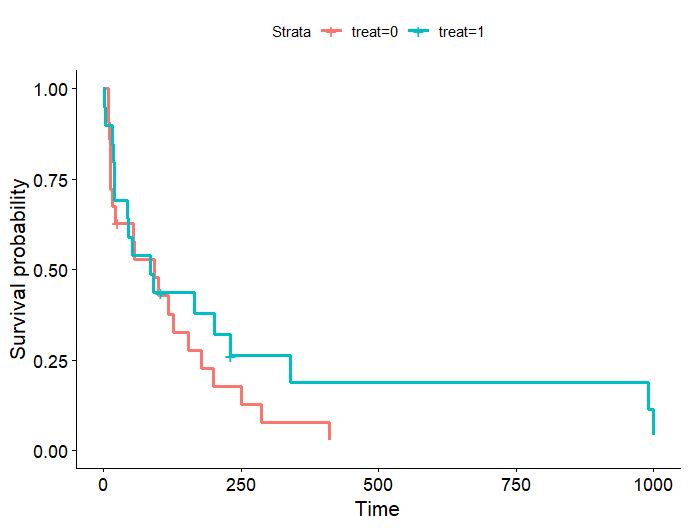
\includegraphics[width=.72\linewidth]{assets/lung_survival.png}\end{center}

\textbf{（2）} 用病理类型1作参照，令 \(I_k=I(type=k)\)： \[\begin{aligned}
h(t\mid X)=h_0(t)\exp\{&-0.614treat-0.001age+0.017coursetime\\&+0.488I_2+1.683I_3+0.264I_4\}.
\end{aligned}\]

\begin{longtable}[]{@{}lrrrl@{}}
\toprule\noalign{}
变量 & \(\beta\) & SE & \(P\) & HR（95\% CI） \\
\midrule\noalign{}
\endhead
\bottomrule\noalign{}
\endlastfoot
试验疗法 & −0.614 & 0.408 & 0.132 & 0.541 (0.244--1.203) \\
年龄 & −0.001 & 0.019 & 0.969 & 0.999 (0.963--1.037) \\
病程 & 0.017 & 0.013 & 0.179 & 1.017 (0.992--1.043) \\
类型2 vs 1 & 0.488 & 0.532 & 0.358 & 1.630 (0.575--4.619) \\
类型3 vs 1 & 1.683 & 0.615 & 0.006 & 5.384 (1.614--17.963) \\
类型4 vs 1 & 0.264 & 0.470 & 0.574 & 1.302 (0.518--3.273) \\
\end{longtable}

\textbf{（3）} 全模型中类型3与类型1的对比有统计学意义。但分类变量整体检验与单个哑变量检验不同，不能直接删除所有不显著项后沿用原系数，声称得到``最终模型''。研究关心的治疗因素应保留。

\textbf{（4）} PH诊断：治疗项Schoenfeld检验 \(P=0.75\)，全局 \(P=0.42\)，未发现显著违反PH的证据。曲线相交只是提示；\(P>0.05\) 不是证明假定成立。全模型似然比9.96（6自由度，\(P\approx0.13\)）、Wald10.28、Score11.23（原稿均约0.1、0.1、0.08）。\(C=0.638\) 表示区分能力有限，C指数不是完整的拟合/校准指标，亦非只在0.5--1之间取值。进一步检查函数形式、影响点、校准与内部验证。

\textbf{（5）} 调整后试验疗法的死亡瞬时风险点估计较低，但区间跨1，未能证实疗效差异；不等于两种疗法等效。可能原因包括样本小、估计不精确、残余混杂或真实差异较小。解释病理类型时明确参照，不能把类型编码直接乘以哑变量系数。


\Answer{H3-2}{hsCRP与死亡风险：文献分析}

\textbf{科学问题。} 可疑急性冠脉综合征患者中，肌钙蛋白之外，轻度升高的hsCRP是否与短期和长期全因死亡相关，并改善预测？

\textbf{变量。} 人口学：出生年份/年龄、性别、种族；临床：首次测量血红蛋白、白细胞、血小板、肌酐、肌钙蛋白、hsCRP等连续指标，以及ICD诊断等分类指标；身份标识：脱敏NHS号、医院号；结局：时间起点、死亡/随访结束时间、死亡状态。\textbf{原稿``死亡日期转换为当日生存率''不准确：个体原始结局应为随访时间和事件指示，生存率是群体估计量。}

\textbf{设计与分析。} 回顾性队列。原评分稿记述5家英国心血管中心源人群257,948人，分析102,337人，中位随访3.3年。hsCRP分为 \(<2\)、2--4.9、5--9.9、10--15 mg/L，以 \(<2\) 为参照。多变量Cox模型估计30天和3年死亡关联的HR及95\% CI。模型1调整年龄、性别、血红蛋白、肌酐；模型2再加肌钙蛋白；模型3再加hsCRP。

原文对PH不成立采用分时段效应：\(<1\)、1--3、3--6、6--12、12--24、24--36个月；连续变量可用限制性立方样条处理非线性。比较区分度、AUROC、NRI、IDI和阴性预测值时，应按原文处理删失与预测时间窗。模型和变量要对应到研究问题，不能只翻译摘要。


\subsection{往年题}

\Answer{R24-M13}{乘积极限法的计算}

\textbf{答案：C。}

条件生存概率连乘：\(\widehat S=(1-2/5)(1-1/3)=\frac35\times\frac23=0.40\)。

\textbf{补写说明。} 原稿第13题整题缺失；本题为新编练习，并非恢复的往年原题。


\Answer{R24-M4}{事件与删失的排序}

\textbf{答案：A。}

A项错误。同一记录时点同时有事件和右删失时，常规KM约定先计事件，后移除删失者；在事件时刻的风险集中包含同刻删失者。

\textbf{补写说明。} 原稿只记一个错误选项，其内容保留为A；提问句及B---E为补写。


\Answer{R24-M5}{生存曲线检验的权重}

\textbf{答案：B。}

按课程相对比较口径，通常选 \textbf{B}：Breslow以风险集人数加权，相对更强调早期；Log-rank相对于Breslow对后期差异保留更多权重。严格地说，不能保证Log-rank总对任意``远期效应''最敏感；其效能取决于生存差异形式，PH下表现良好。

\textbf{补写说明。} 原有五个选项保留；提问句根据回忆内容补全。此处``远期''是相对于Breslow的课程比较。


\Answer{R24-M6}{比例风险与时间}

\textbf{答案：D。}

根据本题已明确的个体风险函数，在共同基线、PH成立且比较的协变量不随时间变化时，\(h(t\mid x_a)/h(t\mid x_b)=\exp\{\beta^T(x_a-x_b)\}\)，与时间无关。若严格指同一模型的共同基线风险函数，其比值就是1。分层Cox不同层基线可不同，不能套用同一结论。

\textbf{补写说明。} 原稿未记选项，并写作``基线风险函数之比''；此处按通常考点将提问对象明确为个体风险函数。


\Answer{R24-M10}{删失与终点事件}

\textbf{答案：A。}

研究终点为肝癌死亡时，\textbf{A}为观察到的事件。B、E属于竞争事件；在原因别风险分析的传统编码中常在竞争死亡时删失，但估计肝癌累计发生概率时需要竞争风险方法。若研究终点为全因死亡，分类会不同。

\textbf{补写说明。} 题干明确了肝癌死亡终点，五个选项保留。


\Answer{R24-D3}{比例风险假设}

固定协变量的两个个体，其风险函数之比不随时间改变：\(HR=\exp\{\beta^T(x_a-x_b)\}\)。允许共同的基线风险 \(h_0(t)\) 随时间变化，并不要求每个人的风险本身恒定。


\Answer{R24-D4}{删失数据}

事件时间只被部分观察到的数据。右删失知道事件时间大于最后观察时间；左删失知道小于某时间；区间删失知道落在某区间。随访结束未发生事件、失访可产生右删失。常规生存估计需适当的非信息性删失假定。


\Answer{Z-D4}{删失数据／截尾数据（Censored data）}

事件时间只获得部分信息。原汇总给的是右删失定义：只知道真实事件时间超过最后观察时间。更一般还包括左删失和区间删失。


\Answer{Z-D5}{比例风险假设（PH Assumption）}

固定协变量个体间的HR不随时间改变；基线风险本身可随时间变化。


\Answer{Z-D6}{风险比（Hazard Ratio, HR）}

同一时刻两种条件下瞬时风险函数之比。Cox模型在PH成立时 \(HR=e^{\beta^T\Delta x}\)；HR不等于累计风险比或OR。


\Answer{R24-S1}{乘积极限法}

有个体事件/删失时间的未分组资料可采用Kaplan--Meier法，不限于小样本。将每个不同事件时刻视为分割点，按条件生存概率连乘： \[\hat S(t)=\prod_{t_i\le t}\left(1-\frac{d_i}{n_i}\right),\] 其中 \(n_i\) 为事件前风险人数，\(d_i\) 为该时刻事件数。可充分利用删失前的信息，不需指定生存时间分布，也不需人为分组；尾部风险人数很少时不稳定，应展示风险人数和区间。


\Answer{R24-S3}{Cox系数与用途}

其他协变量固定、PH成立时，\(X_j\) 增加1单位，瞬时风险乘以 \(e^{\beta_j}\)；\(\beta_j\) 为对应HR的自然对数。分类变量相对参照水平解释，交互项存在时需条件化。用于分析生存时间的关联因素、调整混杂、比较治疗/暴露，以及在模型验证和基线风险估计后预测生存概率。


\Answer{Z-S3}{删失的常见原因}

右删失表示只知道事件时间晚于观察截止。例：随访结束未发生事件、随访期间失访、以特定死因为终点时发生其他死因死亡。第三种同时涉及竞争风险，分析需与目标估计量一致。


\Answer{Z-S4}{KM法与寿命表法}

KM法适用于掌握个体事件/删失时间的原始资料，以每个事件时刻划分风险集，大小样本均可。寿命表法适用于按时间区间汇总的资料，通常需区间内删失分布的近似。原汇编只强调``小样本/大样本''过于简化，关键在记录精度和分组形式。


\Answer{Z-S5}{两种生存曲线检验}

二者比较各组生存经验中的观察/期望事件差异，通常以生存分布相同为无效假设。Log-rank对各事件时刻采用常规等权的观察减期望贡献；Breslow广义Wilcoxon用风险集人数加权，更强调早期。原汇编``Log-rank对远期更敏感''应理解为相对Breslow的课程表述，非普遍定律。


\Answer{Z-S6}{PH假设及其评价}

HR不随时间改变。可看对数负对数生存曲线是否大致平行、检验/绘制缩放Schoenfeld残差，以及检验协变量与时间交互。需同时关注每个变量与全局检验；未拒绝PH不等于证明PH。


\Answer{E19-2}{删失、非比例风险与交互作用}

``截尾''在本课程语境中指删失，即事件时间只有部分信息，右删失时知道 \(T>C\)。严格术语中 truncation（截断）涉及样本被观察到的选择机制，与 censoring不同。

PH不成立可考虑时变系数（协变量与时间交互）、分时段效应、对不关注其系数的变量分层，或根据科学问题改用其他生存模型。应先核对函数形式、异常点及诊断证据。

同时吸烟饮酒与均不者相比，\(HR=e^{0.693+1.099+0.405}\approx9\)；饮酒者中吸烟与不吸烟相比，\(HR=e^{0.693+0.405}\approx3\)。原表写RR，但Cox的指数系数应解释为瞬时风险比HR，不是累计发病概率之比。


\Answer{R24-C2}{心肌梗死风险因素的性别差异}

可能使用Cox比例风险模型，以随访时间和心肌梗死事件指示共同构成生存结局；可处理右删失，无需指定基线风险函数的参数形式，但须检查PH等前提。仅凭HR标签不能排除其他生存模型，应与文献方法核对。

按男女分别报告HR、95\% CI、参照及调整变量。判断性别差异应用性别\(\times\)因素交互作用或等价异质性检验；``男性显著、女性不显著''不等于两者效应差异显著。原图缺失，不能补造具体结论。


\Answer{E19-4}{戒毒方式与复吸时间}

\textbf{整理者复算。} 以 \((time,censor)\) 构成生存结局，模型纳入treat、age、ndrugtx、site、herco；site、herco按分类变量处理。628条原始记录，完整记录610条，495次复吸。长期相对短期：\(\hat\beta=-0.2546\)，HR=0.7752，95\% CI 0.6486--0.9266，\(P=0.00515\)。调整其他变量后，长期方案与较低的复吸瞬时风险相关。

年龄每增1岁HR=0.9765；既往戒毒每增1次HR=1.0354。herco=2相对1的HR=1.2806（\(P=0.0439\)）；site与herco=3对比未达到0.05水平。PH全局检验 \(P=0.318\)，治疗项 \(P=0.092\)，未发现明显违反证据；仍应观察残差图。模型 \(C=0.581\)，预测区分度有限。不要将名为censor的列再次反转编码。


\Answer{E20-3}{冠心病数据分析（2020）}

\textbf{先明确结局。} 原数据的Status只有Alive/Dead，没有死亡原因。因此不能从现有数据直接识别``冠心病特异死亡''。原材料将已确诊冠心病的1449人留下，按确诊后生存时间建模，实际得到的是\textbf{冠心病确诊者后续全因死亡}的分析，不等同于原题的病因特异结局。

\textbf{可复现的示范。} 明示把随访结束近似为基线后32年，确诊者中死亡者时间为``死亡年龄减确诊年龄''，存活者时间为 \(32-(AgeCHDdiag-AgeAtStart)\)。该时间近似用于复现教学分析；若需精确分析，应补齐日期。使用确诊年龄、性别、体重状态、吸烟状态、血压状态、胆固醇状态的Cox模型，参照组为女性、正常体重、不吸烟、理想血压、适宜胆固醇。两年原始表排序不同，但本设定复算均为1405条完整记录、865个死亡事件。

报告系数、HR、95\% CI、PH和共线性诊断；R程序随包提供。原答卷的年龄HR约1.07、男性约1.67、高血压约1.77属于上述全因死亡示例，不能挪作冠心病特异死亡结果。原答卷``偏瘦HR=1.31''与其表中1.98不符；表中BP的PH检验 \(P=0.040\) 也不能被全局 \(P=0.07\) 掩盖。

\textbf{若严格回答原题。} 需要死因或可靠冠心病死亡标志，之后构造病因特异事件、明确竞争事件处理；如果目标是从基线开始的风险分析，亦不能事后仅保留最终确诊者而改变目标人群。


\Answer{E21-3}{冠心病数据分析（2021）}

\textbf{先明确结局。} 原数据的Status只有Alive/Dead，没有死亡原因。因此不能从现有数据直接识别``冠心病特异死亡''。原材料将已确诊冠心病的1449人留下，按确诊后生存时间建模，实际得到的是\textbf{冠心病确诊者后续全因死亡}的分析，不等同于原题的病因特异结局。

\textbf{可复现的示范。} 明示把随访结束近似为基线后32年，确诊者中死亡者时间为``死亡年龄减确诊年龄''，存活者时间为 \(32-(AgeCHDdiag-AgeAtStart)\)。该时间近似用于复现教学分析；若需精确分析，应补齐日期。使用确诊年龄、性别、体重状态、吸烟状态、血压状态、胆固醇状态的Cox模型，参照组为女性、正常体重、不吸烟、理想血压、适宜胆固醇。两年原始表排序不同，但本设定复算均为1405条完整记录、865个死亡事件。

报告系数、HR、95\% CI、PH和共线性诊断；R程序随包提供。原答卷的年龄HR约1.07、男性约1.67、高血压约1.77属于上述全因死亡示例，不能挪作冠心病特异死亡结果。原答卷``偏瘦HR=1.31''与其表中1.98不符；表中BP的PH检验 \(P=0.040\) 也不能被全局 \(P=0.07\) 掩盖。

\textbf{若严格回答原题。} 需要死因或可靠冠心病死亡标志，之后构造病因特异事件、明确竞争事件处理；如果目标是从基线开始的风险分析，亦不能事后仅保留最终确诊者而改变目标人群。


\subsection{补充练习}

\Answer{P3-M1}{时段生存概率与累计生存率}

\textbf{答案：C。} 因为\(\{T>5\}\subset\{T>2\}\)，
\[P(T>5\mid T>2)=\frac{S(5)}{S(2)}=0.75.\]
这是已生存满2年者继续生存至5年的条件概率。\(F(5)=1-S(5)=0.40\)；瞬时风险\(h(5)\)不是\(1-S(5)\)，仅凭两个生存率不能确定。



\Answer{P3-D1}{中位生存期}

中位生存期是生存分布的第50百分位数，即生存函数降至0.5所对应的时间。对阶梯状KM估计，取\(\inf\{t:\hat S(t)\le0.5\}\)，即首次降至0.5或以下的事件时刻。若随访内未降至0.5，应报告“中位生存期尚未达到／在本观察期内不可估计”，不能用最长随访时间或死亡者生存时间的中位数代替。寿命表的分组估计可按正文作线性内插。



\Answer{P3-S1}{删失者如何参与部分似然}

说法错误。删失者在删失之前仍在风险集中，会参与此前事件时刻的分母。

时刻1前，风险集为\(\{\text{甲、乙、丙、丁}\}\)；时刻3前，甲已发生事件、乙已删失，风险集为\(\{\text{丙、丁}\}\)。没有并列事件，故
\[L_p(\beta)=\frac{1}{2+2e^\beta}\times\frac{e^\beta}{1+e^\beta}.\]
例如\(\beta=0\)时，两个贡献为\(1/4\)、\(1/2\)，乘积为\(1/8\)。乙、丁虽没有独立的事件分子，仍提供有效信息。

在同一时刻给定风险集中有人发生事件，某个体的贡献为\(h_i(t)/\sum_{l\in R(t)}h_l(t)\)。各人的共同因子\(h_0(t)\)约去，从而只剩协变量与\(\beta\)。



\Answer{P3-C1}{有并列时间的KM计算}

\textbf{（1）} 事件时刻只有1、2、4月：
\begin{center}\begin{tabular}{rrrr}\toprule
\(t_i\) & \(n_i\) & \(d_i\) & \(\hat S(t_i)\)\\\midrule
1 & 8 & 1 & \(7/8=0.875\)\\
2 & 7 & 1 & \((7/8)(6/7)=0.750\)\\
4 & 4 & 2 & \((3/4)(2/4)=0.375\)\\\bottomrule
\end{tabular}\end{center}
2月的风险集包含同刻删失者；2月后余5人，3月再删失1人，所以4月前余4人。

\textbf{（2）} \(\hat S(3)=0.750\)、\(\hat S(4)=0.375\)。首次降至0.5以下为4月，中位生存期为4月。删失不会直接使曲线下降，而会改变之后的风险人数；5、6月的删失也不会把末尾生存率降为0。

\textbf{（3）}
\[SE\{\hat S(4)\}=0.375\sqrt{\frac1{8\times7}+\frac1{7\times6}
+\frac2{4\times2}}=0.2025.\]
不能把已删失者一开始就剔除，也不能在2月先移除删失者再计算死亡概率。



\Answer{P3-C2}{寿命表与中位生存期的内插}

\textbf{（1）} 有效人数为\(n_i=n_i'-c_i/2\)，条件生存概率为\(p_i=1-d_i/n_i\)：
\begin{center}\begin{tabular}{lrrr}\toprule
区间 & 有效人数 & \(p_i\) & 区间末\(\hat S\)\\\midrule
0--1 & 90 & 0.80 & 0.80\\
1--2 & 50 & 0.80 & 0.64\\
2--3 & 28 & 0.75 & 0.48\\\bottomrule
\end{tabular}\end{center}
期初人数递推也自洽：\(100-18-20=62\)，\(62-10-24=28\)。

\textbf{（2）} 0.5位于2年和3年的生存率之间，内插为
\[\hat t_{0.5}=2+\frac{0.64-0.50}{0.64-0.48}(3-2)=2.875\text{年}.\]
这是分组资料下的近似，不能当作精确事件时刻。

\textbf{（3）} 0.75的条件是已经生存至第3个区间开始，而3年生存率须累乘前面各区间，得到\(0.8\times0.8\times0.75=0.48\)。原表缺少区间内事件、删失的确切时间与顺序，不能唯一还原KM曲线。



\Answer{P3-C3}{从预后指数计算生存率}

\textbf{（1）} 基线对应50岁、标准疗法。60岁试验组患者有
\[PI=\log0.5+\log1.5=\log0.75=-0.2877,\quad HR=e^{PI}=0.75.\]
年龄是按每10岁进入方程，不能把60直接乘以年龄系数。

\textbf{（2）} 由正文公式\(\hat S(t\mid X)=\hat S_0(t)^{e^{PI}}\)，得
\[\hat S(3\mid X)=0.64^{0.75}=0.7155.\]
HR作用于风险函数；在生存函数中进入\textbf{指数}，不能计算成\(0.64\times0.75\)。

\textbf{（3）} 相同年龄比较两疗法，\(HR=0.5\)。60岁标准组的3年生存率为\(0.64^{1.5}=0.512\)，故本例3年累计死亡概率之比为
\[\frac{1-0.7155}{1-0.512}\approx0.5829,\]
与0.5不同。HR是同一时刻瞬时风险之比，不是指定随访期限的累计死亡概率之比。



\Answer{P3-L1}{体育活动、死亡终点与剂量反应}

\textbf{（1）} 个体结局由随访时间与事件指示共同构成。时间从规定基线至死亡、失访或随访截止；以全因死亡为终点，癌症死亡也记事件1，而非删失0。换成死因别终点时需重新定义事件及其他死因的处理。

\textbf{（2）} 在模型调整因素相同并满足其假定时，75--149分钟/周组全因死亡瞬时风险为参照组的0.81倍，即相对低19\%；95\% CI为0.76--0.87，未跨1。心血管疾病死亡的HR为0.69，即相应瞬时风险低31\%，95\% CI为0.60--0.78。它们不表示30年死亡概率下降相同的百分点，也不能仅凭观察性关联断言运动干预造成同样幅度的下降。

\textbf{（3）} 限制性立方样条用于描述连续运动时长与对数风险之间可能的\textbf{非线性剂量反应关系}。PH关注效应是否随随访时间变化，是另一项问题，仍需另行评价。高运动量端趋平提示增加运动时长的额外关联可能减弱；还应结合置信区间和该段数据量，不能只凭曲线宣布某一剂量绝对最优。
\EndExercises
